\documentclass[11pt]{article}

% ---------------------------------------------------------------------------
%  Parallelising timed-automata reachability: OpenMP and Metal GPU backends
% ---------------------------------------------------------------------------
\usepackage[utf8]{inputenc}
\usepackage[T1]{fontenc}
\usepackage{lmodern}
\usepackage[a4paper,margin=2.4cm]{geometry}
\usepackage{amsmath,amssymb,amsthm}
\usepackage{booktabs}
\usepackage{xcolor}
\usepackage{graphicx}
\usepackage{caption}
\usepackage{subcaption}
\usepackage{algorithm}
\usepackage{algpseudocode}
\usepackage{listings}
\usepackage{microtype}
\usepackage{tikz}
\usepackage{pgfplots}
\pgfplotsset{compat=1.18}
\usetikzlibrary{arrows.meta,positioning,calc,fit,backgrounds,shapes.geometric,
                decorations.pathreplacing,shadows.blur,matrix}
\usepackage[hidelinks]{hyperref}
\usepackage[nameinlink]{cleveref}

% ---- palette --------------------------------------------------------------
\definecolor{cpu}{HTML}{2C6E9B}     % blue   -- host / CPU
\definecolor{gpu}{HTML}{B5651D}     % orange -- GPU
\definecolor{acc}{HTML}{3F7A3F}     % green  -- accents
\definecolor{soft}{HTML}{F1F4F8}
\definecolor{softg}{HTML}{FBEFE3}
\definecolor{codebg}{HTML}{F7F7F4}

% ---- tikz styles ----------------------------------------------------------
\tikzset{
  box/.style   ={rounded corners=2pt, draw=black!55, thick, align=center,
                 font=\small, inner sep=5pt, minimum height=8mm},
  cpubox/.style={box, fill=soft,  draw=cpu!70},
  gpubox/.style={box, fill=softg, draw=gpu!75},
  lane/.style  ={rounded corners=3pt, draw=black!25, thick, inner sep=7pt},
  flow/.style  ={-{Stealth[length=2.4mm]}, thick, draw=black!65},
  dflow/.style ={-{Stealth[length=2.4mm]}, thick, draw=black!45, dashed},
  lbl/.style   ={font=\scriptsize\itshape, text=black!60},
}

% ---- listings -------------------------------------------------------------
\lstset{
  basicstyle=\ttfamily\footnotesize, backgroundcolor=\color{codebg},
  breaklines=true, columns=fullflexible, keepspaces=true, frame=single,
  rulecolor=\color{black!20}, framesep=4pt, xleftmargin=4pt,
  commentstyle=\color{acc}, keywordstyle=\color{cpu}\bfseries,
  language=C++, showstringspaces=false, morekeywords={kernel,device,__global__,constant,thread}
}

\newtheorem{proposition}{Proposition}
\newcommand{\dk}{\ensuremath{\mathit{dk}}}
\newcommand{\aluleq}{\ensuremath{\preceq_{\mathrm{aLU}}}}
\newcommand{\code}[1]{\texttt{\small #1}}

\title{\bfseries Parallelising Timed-Automata Reachability:\\[2pt]
  \large A Shared-Memory (OpenMP) and a GPU (Metal/CUDA) Backend for a Timed-CTL Model Checker}
\author{PTCTLMC Project}
\date{\today}

\begin{document}
\maketitle

\begin{abstract}
\noindent
We describe two parallel backends for the reachability engine of \textsc{PTCTLMC}, a model
checker for timed automata and networks thereof. The engine explores a \emph{zone graph}:
symbolic states pair a discrete location/variable vector with a convex \emph{zone} of clock
valuations, represented as a Difference Bound Matrix (DBM). Two operations dominate the cost:
computing successor zones, and merging them into a \emph{passed list} under
abstraction-based subsumption and exact convex union. Both are embarrassingly parallel
\emph{across} symbolic states but stubbornly sequential \emph{within} a merge bucket.
Our first backend shards the passed list by a packed discrete key and lets OpenMP workers
expand the frontier and merge disjoint shards without locks. Our second backend runs the entire
level loop on an Apple Metal GPU: one GPU thread per successor ``recipe'' and one GPU thread per
discrete-state bucket, with a host-side marshaling layer that we ultimately parallelise across the
CPU cores as well---so the machine computes with the GPU \emph{and} all cores at once. We validate
that every backend explores the \emph{identical} zone graph as UPPAAL---matching its stored- and
explored-state counts \emph{integer-for-integer} on Fischer, two-lock and arbiter---so the
speed-ups compare like with like. Across an evaluation whose per-model size grid is capped by the
machine's memory ceiling, both parallel backends beat single-threaded \texttt{verifyta} on every
model (OpenMP by up to $3.5\times$). The Metal backend additionally beats the 12-thread OpenMP
backend on the \emph{expansion-dominated} models---Fischer, two-lock and arbiter---reaching
$3.3$--$6.2\times$ over \texttt{verifyta}; a single optimisation that stops the host copying freshly
generated zones (the merge kernel reads them in place from the expand kernel's output) is what turns
the largest Fischer instance from a loss into a win. The one place the naive GPU merge \emph{loses}---a
\emph{merge-dominated} model (dining philosophers), where its one-thread-per-bucket kernel is the
wrong shape and collapses to $122$\,s---we \emph{fix} with an \code{--adaptive} mode that calibrates
the GPU-versus-12-core-CPU merge throughput per level and routes each level to the faster path: a
$14$--$47\times$ speed-up that makes the adaptive Metal backend the fastest configuration on
\emph{every} model, beating OpenMP throughout and \code{verifyta} by $3.4$--$7.3\times$. Its cost is
memory---the GPU backends carry a double-buffering premium---so peak RAM, not run time, sets the
ceiling on a $24$\,GB laptop. We give the design, intuition and diagrams for both backends, an honest
account of three optimisations that \emph{failed}, and a CUDA port that inherits the adaptive merge for
datacentre GPUs.
\end{abstract}

% ===========================================================================
\section{Introduction}
% ===========================================================================
A \emph{timed automaton} is a finite automaton equipped with real-valued clocks that advance
synchronously and can be compared against integer constants and reset on transitions. Verifying
a property such as \emph{``two processes are never simultaneously in their critical
section''} reduces to a reachability question over an infinite state space (locations $\times$
clock valuations in $\mathbb{R}_{\geq 0}^{n}$). The classical solution replaces sets of clock
valuations by \emph{zones}---convex polyhedra defined by difference constraints
$x_i - x_j \bowtie c$---and explores the resulting \emph{zone graph}, which can be kept finite by
sound abstractions. Real benchmarks (Fischer mutual exclusion, CSMA/CD, train--gate) are
\emph{networks} of such automata communicating through shared bounded integer variables and
synchronisation channels; their product state spaces explode combinatorially, and this is exactly
where wall-clock time is spent.

\textsc{PTCTLMC} is a from-scratch checker whose reference (sequential) engine is validated against
UPPAAL. This report concerns \emph{how we made it fast in parallel}, on two very different pieces of
hardware:
\begin{itemize}\itemsep2pt
  \item a \textbf{shared-memory} backend using \textbf{OpenMP} across CPU cores
        (\cref{sec:omp}); and
  \item a \textbf{GPU} backend using Apple \textbf{Metal} (\cref{sec:metal}), mirrored to
        \textbf{CUDA} for datacentre GPUs (\cref{sec:cuda}).
\end{itemize}
Both share one control structure---a level-synchronised breadth-first search---and the same
correctness oracle. We foreground \emph{intuition}: what is being computed, where the parallelism
comes from, and why a natural-looking optimisation can make things slower. All diagrams are
TikZ-drawn and every performance number is reproducible with the benchmark generators shipped in
\code{benchmarks/}.

% ===========================================================================
\section{Background: the zone graph and where time goes}\label{sec:bg}
% ===========================================================================
A \emph{symbolic state} of a network is a pair $s = (\ell, Z)$ where
$\ell = (\ell_1,\dots,\ell_p, v_1,\dots,v_m)$ is the \emph{discrete part} (one location per process
plus the shared integer variables) and $Z$ is a \emph{zone} over the $n$ shared clocks. A zone is
stored as a \emph{Difference Bound Matrix} (DBM): an $(n{+}1)\times(n{+}1)$ matrix $D$ whose entry
$D_{ij}$ is the tightest bound on $x_i - x_j$ (index $0$ is a fixed zero clock), each bound
encoded as a single machine integer $(\text{value}\,{\ll}\,1)\,|\,\text{strict}$. Every zone
operation---intersection with a guard, clock reset, time-elapse (``delay''), emptiness---is a
handful of nested loops over $D$ and runs identically on CPU and GPU
(\cref{fig:dbm}).

\begin{figure}[t]
\centering
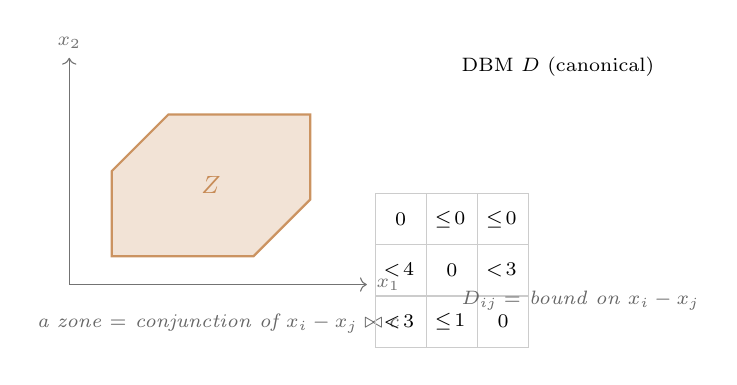
\begin{tikzpicture}[scale=0.9]
  % clock plane
  \draw[->,black!55] (0,0) -- (4.2,0) node[right]{\scriptsize $x_1$};
  \draw[->,black!55] (0,0) -- (0,3.2) node[above]{\scriptsize $x_2$};
  \fill[gpu!18,draw=gpu!70,thick] (0.6,0.4) -- (2.6,0.4) -- (3.4,1.2) -- (3.4,2.4)
       -- (1.4,2.4) -- (0.6,1.6) -- cycle;
  \node[gpu!75] at (2.0,1.4) {\small $Z$};
  \node[lbl,align=left] at (2.1,-0.55)
       {\scriptsize a zone $=$ conjunction of $x_i-x_j \bowtie c$};
  % DBM
  \begin{scope}[xshift=5.4cm,yshift=0.2cm]
    \node[anchor=south west] at (0,2.6) {\scriptsize DBM $D$ (canonical)};
    \matrix (m) [matrix of nodes, nodes={draw=black!20, minimum size=6.5mm,
        font=\scriptsize, anchor=center}, column sep=-\pgflinewidth, row sep=-\pgflinewidth]
    {
      $0$ & $\!\le\!0$ & $\!\le\!0$ \\
      $\!<\!4$ & $0$ & $\!<\!3$ \\
      $\!<\!3$ & $\!\le\!1$ & $0$ \\
    };
    \node[lbl,anchor=north west] at (0,-0.15)
      {\scriptsize $D_{ij}=$ bound on $x_i-x_j$};
  \end{scope}
\end{tikzpicture}
\caption{A clock zone and its DBM. All backends manipulate the DBM with the \emph{same}
\code{\_\_host\_\_ \_\_device\_\_} operations, so GPU code runs CPU-validated algebra.}
\label{fig:dbm}
\end{figure}

\paragraph{The level-synchronised loop.} Reachability is a breadth-first exploration of the zone
graph organised in \emph{levels} (\cref{fig:loop}). Starting from the initial symbolic state, each
iteration (i)~\emph{expands} the current frontier---applies every enabled transition to every
frontier state to produce successor zones---and (ii)~\emph{merges} those successors into a
\emph{passed list} keyed by discrete state, keeping only an \emph{antichain} of maximal zones per
key. Survivors of the merge form the next frontier. The property holds/fails as soon as a target
state is generated or the frontier empties.

\begin{figure}[t]
\centering
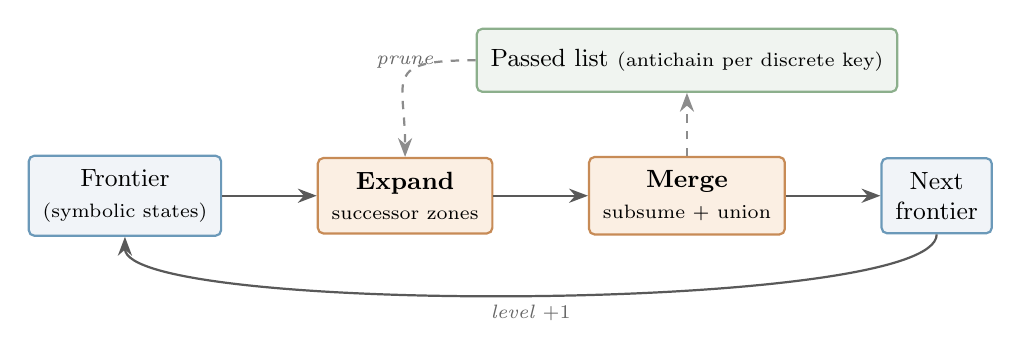
\begin{tikzpicture}[node distance=6mm and 12mm]
  \node[cpubox] (front) {Frontier\\\scriptsize (symbolic states)};
  \node[gpubox, right=of front] (exp) {\textbf{Expand}\\\scriptsize successor zones};
  \node[gpubox, right=of exp] (mrg) {\textbf{Merge}\\\scriptsize subsume $+$ union};
  \node[cpubox, right=of mrg] (nf) {Next\\frontier};
  \draw[flow] (front) -- (exp);
  \draw[flow] (exp) -- (mrg);
  \draw[flow] (mrg) -- (nf);
  \draw[flow] (nf.south) .. controls +(0,-1.0) and +(0,-1.0) .. (front.south)
        node[midway,below,lbl]{level $+1$};
  \node[cpubox, above=8mm of mrg, fill=acc!8, draw=acc!60] (pl)
        {Passed list \scriptsize (antichain per discrete key)};
  \draw[dflow] (mrg) -- (pl);
  \draw[dflow] (pl.west) .. controls +(-1.2,0) and +(0,1.0) .. (exp.north)
        node[midway,above,lbl]{prune};
\end{tikzpicture}
\caption{One iteration of the level-synchronised BFS. \emph{Expand} and \emph{merge} dominate the
runtime; both parallelise across states, and are the targets of \cref{sec:omp,sec:metal}.}
\label{fig:loop}
\end{figure}

\paragraph{The two hot operations.}
\emph{Expansion} is uniform, data-parallel arithmetic: one independent DBM pipeline per
(frontier-state, transition). \emph{Merging} is where subtlety lives. For each discrete key we
maintain an antichain under the \emph{$\text{aLU}$ preorder} \aluleq{}---the abstraction-based
simulation of Herbreteau–Srivathsan–Walukiewicz that is strictly coarser than zone inclusion and
so prunes far more---plus an \emph{exact convex union}: if two stored zones' union happens to be
convex, they are fused into one, which is what collapses the stored-state count to match UPPAAL.
Both tests are $O(\dim^2)$--$O(\dim^3)$ DBM comparisons; a discrete key with $k$ stored zones costs
$O(k^2)$ of them. The antichain per key is small, but there are millions of keys.

\paragraph{The discrete key.} To index the passed list we pack the whole discrete part into a
single 64-bit integer: a fixed bit-field per process location and per integer variable
(\cref{fig:key}). This mirrors UPPAAL's ``compressed integers'' and turns key comparison and
hashing into single-word operations---essential once keys are compared billions of times. The
field widths come from the declared ranges (\code{int[lo,hi]}); getting them wrong silently
collides distinct states (a real bug we found and fixed).

\begin{figure}[t]
\centering
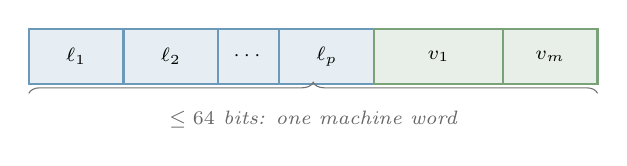
\begin{tikzpicture}[x=0.86cm]
  \foreach \i/\w/\c/\t in {0/1.4/cpu/{$\ell_1$}, 1/1.4/cpu/{$\ell_2$}, 2/1.4/cpu/{$\cdots$},
                            3/1.4/cpu/{$\ell_p$}, 4/1.8/acc/{$v_1$}, 5/1.4/acc/{$\cdots$}} {}
  \def\x{0}
  \foreach \w/\c/\t in {1.4/cpu/{$\ell_1$},1.4/cpu/{$\ell_2$},0.9/cpu/{$\cdots$},1.4/cpu/{$\ell_p$},
                        1.9/acc/{$v_1$},1.4/acc/{$v_m$}} {
    \draw[fill=\c!12,draw=\c!70,thick] (\x,0) rectangle ++(\w,0.7);
    \node at (\x+\w/2,0.35) {\scriptsize \t};
    \pgfmathsetmacro\x{\x+\w}\xdef\x{\x}
  }
  \draw[decorate,decoration={brace,amplitude=4pt},black!55]
     (0,-0.12) -- node[below=3pt,lbl]{$\le 64$ bits: one machine word} (\x,-0.12);
\end{tikzpicture}
\caption{The packed discrete key \dk{}: locations (blue) and bounded integers (green) laid out in
disjoint bit-fields. Hashing/comparing a symbolic state's discrete part is now one word op.}
\label{fig:key}
\end{figure}

% ===========================================================================
\section{The OpenMP backend}\label{sec:omp}
% ===========================================================================
The shared-memory backend keeps the sequential control flow and parallelises the two hot phases
across cores. The design principle is \emph{ownership without locks}: partition the work so that
no two threads ever touch the same passed-list bucket.

\paragraph{Sharding by discrete key.} We split the passed list into $S$ shards (one per worker) by
hashing the discrete key: shard$(\dk) = (\dk \cdot \phi) \bmod S$. Because a given discrete state
always lands in the same shard, each shard is a \emph{self-contained} antichain owned by exactly
one thread during the merge---so the $O(k^2\,\dim^3)$ convex-merge runs fully in parallel with no
synchronisation (\cref{fig:omp}).

\begin{figure}[t]
\centering
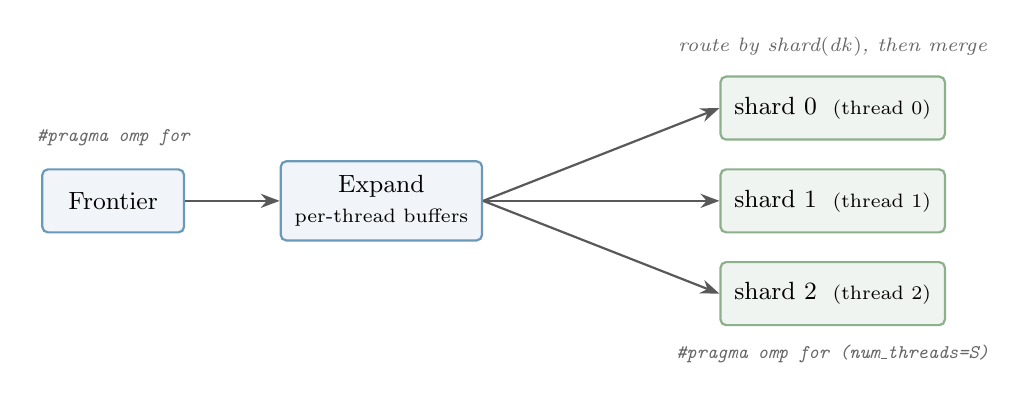
\begin{tikzpicture}
  \node[cpubox,minimum width=18mm] (fr) {Frontier};
  \node[lbl,above=1.6mm of fr] {\ttfamily \#pragma omp for};
  \node[cpubox,right=12mm of fr,minimum width=22mm] (exp)
     {Expand\\\scriptsize per-thread buffers};
  \draw[flow] (fr) -- (exp);
  % shards stacked well to the right; expand fans out into them
  \node[cpubox, fill=acc!8, draw=acc!60, minimum width=26mm, right=30mm of exp] (sh1)
     {shard 1\; \scriptsize(thread 1)};
  \node[cpubox, fill=acc!8, draw=acc!60, minimum width=26mm, above=3.5mm of sh1] (sh0)
     {shard 0\; \scriptsize(thread 0)};
  \node[cpubox, fill=acc!8, draw=acc!60, minimum width=26mm, below=3.5mm of sh1] (sh2)
     {shard 2\; \scriptsize(thread 2)};
  \draw[flow] (exp.east) -- (sh0.west);
  \draw[flow] (exp.east) -- (sh1.west);
  \draw[flow] (exp.east) -- (sh2.west);
  \node[lbl, above=1.2mm of sh0] {route by shard$(\dk)$, then merge};
  \node[lbl, below=1.2mm of sh2] {\ttfamily \#pragma omp for (num\_threads=S)};
\end{tikzpicture}
\caption{OpenMP parallelisation. Workers expand the frontier into private buffers, successors are
routed to shards by a hash of the discrete key, and each shard---a disjoint slice of the passed
list---is merged by a single owning thread. No locks are needed anywhere.}
\label{fig:omp}
\end{figure}

\paragraph{Allocator contention is the real enemy.} A subtle lesson: with the merge correctly
parallelised, scaling still collapsed at large $N$ (from ${\sim}3.6\times$ to ${\sim}1.8\times$ on
12 cores). Profiling showed the culprit was not the algorithm but \code{malloc}: every churned
zone is a \code{malloc}/\code{free} pair, and \code{malloc} holds a \emph{process-global} lock, so
all workers serialised on the allocator. Replacing zone storage with a \emph{per-thread free-list
pool} (recycling equally-sized DBM buffers without touching the global heap) restored scaling. The
message generalises to the GPU: \emph{the bottleneck is rarely the compute; it is the memory
plumbing around it.}

\Cref{alg:omp} summarises the level loop; each \textbf{parallel-for} is a barrier, and the routing
step in between is cheap serial bookkeeping.

\begin{algorithm}[t]
\caption{OpenMP level loop (one iteration)}\label{alg:omp}
\begin{algorithmic}[1]
\State \textbf{parallel for} $s \in \text{frontier}$: \Comment{expand}
       $\text{tls}[\text{tid}] \mathrel{+}= \Call{Successors}{s}$
\For{$s \in \text{tls}[\cdot]$} \Comment{route (serial, cheap)}
   \State \textbf{if} \Call{IsTarget}{$s$} \textbf{return} true
   \State $\text{byshard}[\,\text{shard}(\dk_s)\,] \mathrel{+}= (\dk_s, s)$
\EndFor
\State \textbf{parallel for} $t \in [0,S)$: \Comment{merge disjoint shards}
\State \quad \textbf{for} $(\dk,s) \in \text{byshard}[t]$: \Call{AddTo}{$\text{shard}[t],\,\dk,\,s$}
\State \quad collect this level's survivors into next frontier
\end{algorithmic}
\end{algorithm}

% ===========================================================================
\section{The Metal GPU backend}\label{sec:metal}
% ===========================================================================
GPUs excel at the uniform arithmetic of expansion, but the merge---branchy, data-dependent,
antichain-shaped---is exactly what GPUs are \emph{bad} at. The engineering question is therefore
not ``can the DBM math run on the GPU'' (it can) but ``can we keep the GPU fed without drowning in
host$\leftrightarrow$device traffic.'' Our answer has three ingredients: a \emph{recipe}-based
expand kernel, a \emph{one-thread-per-bucket} merge kernel, and a flat, unified-memory data path
whose host-side plumbing is itself parallelised over the CPU cores.

\subsection{Expand: one GPU thread per successor recipe}
A network transition can be a plain location step, a binary handshake ($a!\,\|\,a?$), or a
broadcast ($a!$ with all enabled $a?$). We unify these as a \emph{recipe}: a short list of
participating $(\text{process},\text{edge})$ pairs. The host enumerates recipes---this is the
discrete part of successor generation (channel matching, integer guards, committed-location
filtering), which is cheap and irregular---while the GPU runs the \emph{zone} pipeline for each
recipe in one thread (\cref{fig:metal}, left): intersect all participants' guards, apply all
resets, intersect the combined target invariant, elapse time unless a participant is
urgent/committed, reset clocks no process can still read, test emptiness. One thread, one
successor zone.

\subsection{Merge: one GPU thread per discrete-state bucket}
After expansion, successors are grouped by discrete key on the host (integer hashing, cheap). Each
\emph{bucket}---the new zones sharing a key, plus that key's existing antichain---is handed to a
single GPU thread that replicates the sequential \code{AddTo} \emph{exactly}: aLU-subsume the new
zone against the stored ones (and vice-versa), attempt convex union, append if it survived. The
work is sequential \emph{within} a bucket (antichains are tiny) and massively parallel \emph{across}
the thousands of simultaneously-touched buckets (\cref{fig:metal}, right). Crucially the convex
union is done on the GPU too---no shortcut---so the stored-state count matches UPPAAL bit for bit.

\begin{figure*}[t]
\centering
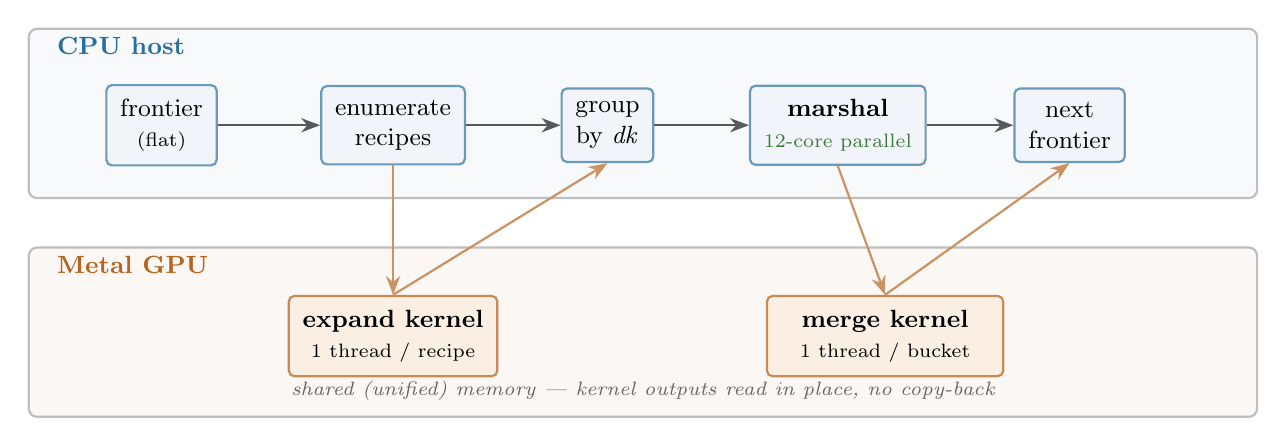
\begin{tikzpicture}[node distance=5mm and 10mm]
  % ---- HOST lane ----
  \node[lane, fill=cpu!4, minimum width=15.6cm, minimum height=2.15cm] (hostlane) {};
  \node[anchor=north west, font=\small\bfseries, text=cpu] at (hostlane.north west) {\ \ CPU host};
  % ---- GPU lane ----
  \node[lane, fill=gpu!5, minimum width=15.6cm, minimum height=2.15cm,
        below=6mm of hostlane] (gpulane) {};
  \node[anchor=north west, font=\small\bfseries, text=gpu] at (gpulane.north west) {\ \ Metal GPU};

  % host boxes
  \node[cpubox] (fr) at ([xshift=1.7cm,yshift=-0.15cm]hostlane.west) {frontier\\\scriptsize (flat)};
  \node[cpubox, right=13mm of fr] (enum) {enumerate\\recipes};
  \node[cpubox, right=12mm of enum] (grp) {group\\by \dk};
  \node[cpubox, right=12mm of grp] (mar)
     {\textbf{marshal}\\\scriptsize \color{acc}12-core parallel};
  \node[cpubox, right=11mm of mar] (nf) {next\\frontier};

  % gpu boxes
  \node[gpubox, minimum width=26mm] (kexp) at ([yshift=-0.05cm]enum|-gpulane)
     {\textbf{expand kernel}\\\scriptsize 1 thread / recipe};
  \node[gpubox, minimum width=30mm] (kmrg) at ([xshift=6mm,yshift=-0.05cm]mar|-gpulane)
     {\textbf{merge kernel}\\\scriptsize 1 thread / bucket};

  % flows
  \draw[flow] (fr) -- (enum);
  \draw[flow] (enum) -- (grp);
  \draw[flow] (grp) -- (mar);
  \draw[flow] (mar) -- (nf);
  \draw[flow, gpu!70] (enum.south) -- (kexp.north);
  \draw[flow, gpu!70] (kexp.north) -- (grp.south);
  \draw[flow, gpu!70] (mar.south) -- (kmrg.north);
  \draw[flow, gpu!70] (kmrg.north) -- (nf.south);
  \node[lbl, anchor=south] at ([yshift=1mm]gpulane.south) {shared (unified) memory --- kernel outputs read in place, no copy-back};
\end{tikzpicture}
\caption{The Metal level loop. The GPU runs the two kernels (expand over recipes, merge over
buckets); the host does only the irregular discrete work (enumeration, grouping) and the zone
\emph{marshalling}, which we parallelise across all CPU cores. Buffers live in unified memory, so
kernel outputs are read \emph{in place} rather than copied back---the machine uses the GPU and all
CPU cores simultaneously.}
\label{fig:metal}
\end{figure*}

\subsection{Keeping the GPU fed: the flat unified-memory data path}
The first working version was three times \emph{slower} than OpenMP, and the profiler explained
why: the GPU kernels were ${\sim}25\%$ of the time, and the remaining ${\sim}75\%$ was the host
converting between \code{SymState} objects and flat arrays, allocating hundreds of megabytes of
Metal buffers \emph{every level}, and copying each zone five or six times. We rebuilt the data path
around four ideas, each validated by re-profiling:
\begin{enumerate}\itemsep2pt
  \item \textbf{Flat, resident state.} No per-state objects; the frontier and passed list are flat
        \code{raw\_t} arrays. This removed a per-successor heap allocation and a map rebuilt from
        \code{Dbm} copies every level.
  \item \textbf{Persistent buffers, written in place.} Apple GPUs share memory with the CPU
        (\emph{unified memory}). We keep grow-on-demand \code{MTLBuffer}s and \emph{gather directly
        into their contents}, so there is no separate ``upload''; symmetrically, kernel outputs are
        read straight from the buffer (\code{const raw\_t*\&} out-parameters), with no read-back
        copy.
  \item \textbf{Parallel host marshalling.} The remaining per-bucket gather/rebuild is over
        independent buckets, so it runs under \code{\#pragma omp parallel for}. The metal backend is
        thus \emph{GPU $+$ 12 cores}, versus OpenMP's 12 cores---strictly more hardware in flight.
  \item \textbf{New-zone gather elimination.} Even after the above, the host still touched every
        freshly generated (``new'') zone \emph{twice}: once to stage it into the merge's work buffer,
        once to read the merged result back. We removed the first pass entirely: the merge kernel
        reads new zones \emph{in place} from the expand kernel's output buffer, indexed by a
        \code{new\_idx} array, so the host stages only each key's \emph{existing} antichain. This
        halved the host memcpy profile and, on Fischer $N{=}12$, turned a ${\sim}17.6$\,s \emph{loss}
        to OpenMP into a ${\sim}12.2$\,s \emph{win}---the single change that makes Metal beat the CPU
        across the expansion-dominated models (\cref{sec:eval}).
\end{enumerate}
A final micro-optimisation: a bucket all of whose new zones are subsumed is \emph{unchanged}, so we
skip its rebuild and frontier gather entirely.

\begin{lstlisting}[caption={The merge output is read in place from unified memory---no copy.},captionpos=b]
// bucket b's final antichain, straight from the GPU buffer:
for (int i = 0; i < out_count[b]; ++i) {
  const raw_t* z = out_zones + (work_off[b]+i)*d2;
  if (out_isnew[work_off[b]+i]) /* -> next frontier */;
}
\end{lstlisting}

\subsection{Two optimisations that failed (and why)}
Intuition said the ultimate win was a \emph{GPU-resident arena}: keep every passed-list zone on the
GPU forever, store only \code{dk -> (offset,count)} on the host, and have the merge read existing
zones \emph{in place} from the arena---eliminating even the existing-zone gather. We implemented it
fully and it was \emph{exact-correct}, yet it \emph{regressed} every problem size. Two reasons,
both instructive: (i) the kernel must still copy each bucket's existing antichain into a fresh
append region, and that copy now runs \emph{single-threaded per bucket on the GPU} instead of
across 12 CPU cores; and (ii) an append-only arena needs periodic compaction, a multi-gigabyte host
\code{memmove}. A second attempt---writing each level's next frontier \emph{directly} into a
persistent GPU buffer instead of gathering it---also regressed (Fischer $N{=}12$: $12.2\!\to\!14.0$\,s),
because it turned one large \emph{sequential} gather into many \emph{scattered} host writes into
GPU-shared memory, which are slow once the working set is large. We reverted both. The lesson is the
recurring theme of this report: on a memory-bound workload, moving a copy onto slower hardware---or
scattering it---loses even when it removes a copy.

\subsection{Adaptive merge routing: CPU or GPU, chosen per level}\label{sec:adaptive}
The one-thread-per-bucket merge is the \emph{right} shape only when a level has \emph{many, thin}
buckets: on Fischer, ${\sim}70$k buckets each hold a tiny antichain, so thousands of GPU lanes each do
a little work. It is the \emph{wrong} shape when the per-bucket work is heavy. On dining philosophers
the exact convex union fires constantly, each of a few thousand buckets carries an $O(k^2\dim^3)$
load, and a handful of weak GPU lanes grind through it while the CPU cores idle. The profiler is
unambiguous: the merge kernel is ${\approx}\,93\%$ of the Metal wall-clock on philosophers versus
${\approx}\,31\%$ on Fischer. Tellingly, \emph{static} bucket-size heuristics (bucket count,
mean/max antichain size) do \emph{not} separate the two cases---the discriminator is the branchy
convex-union cost, which those metrics cannot see. So the driver \emph{measures} rather than guesses.

With the \code{--adaptive} flag, the flat driver keeps a host port of the merge kernel,
\code{flat\_merge\_bucket}, that runs the identical aLU-subsumption and convex-union on the CPU using
the very same \code{\_\_host\_\_ \_\_device\_\_} \code{dbm\_ops} routines, parallelised across buckets
with \code{\#pragma omp parallel for}---i.e. the merge on all 12 cores instead of one GPU thread each.
For every BFS level it estimates the merge work as $\sum_b |\mathrm{bucket}_b|^2$ and records each
path's \emph{throughput} (work per millisecond); it calibrates the CPU path first (never
catastrophic), then the GPU path, then routes every subsequent level to whichever is \emph{measured}
faster, updating the estimate as it goes. \emph{Expansion always stays on the GPU}---only the merge is
routed. Because this lives in the \emph{shared} flat driver and not in device code, the CUDA backend
(\cref{sec:cuda}) inherits it unchanged.

The default stays the naive one-thread-per-bucket merge; \code{--adaptive} is opt-in. The effect is
large where it matters and harmless elsewhere: on philosophers $N{=}11$ the Metal wall-clock drops
from $8.1$\,s to $0.6$\,s---a $13\times$ speed-up that turns the backend's \emph{worst loss} into a
win over both the 12-thread OpenMP backend ($1.2$\,s) and \code{verifyta} ($2.6$\,s)---while the
already-merge-light Fischer still improves slightly ($2.64\!\to\!2.31$\,s). The pathology is
GPU-specific: OpenMP's merge is \emph{already} parallel across buckets (\cref{sec:omp}), so it has
nothing to route---an \code{omp} ``adaptive'' mode would toggle nothing.

% ===========================================================================
\section{The CUDA port}\label{sec:cuda}
% ===========================================================================
Because the \emph{control} of the level loop lives in host code and only the \emph{device} layer is
platform-specific, porting to CUDA is a device-for-device exercise. The CUDA backend
(\code{netengine\_cuda.cu}) reuses the shared network encoding and the \emph{same}
\code{\_\_host\_\_ \_\_device\_\_} DBM operations the CPU is tested on, so the kernels---one
\code{net\_expand} over recipes, one \code{net\_merge} over buckets---are line-for-line twins of the
Metal shaders. The unified-memory data path maps onto CUDA \emph{managed} memory
(\code{cudaMallocManaged}), which lets the very same host driver write merge inputs and read outputs
through raw pointers. Datacentre GPUs (H100) have both far higher arithmetic throughput and much
wider memory bandwidth---and thousands more lanes---which are precisely the resources that bound the
laptop GPU at the two places it currently \emph{loses} (\cref{sec:eval}): the memory-bound top of the
scaling curve, and the merge-heavy models where a wider machine would let a threadgroup-per-bucket
merge parallelise the antichain scan instead of stalling one lane per bucket. We therefore expect the
CUDA backend both to raise the ceiling and to soften the merge-dominated worst case.

% ===========================================================================
\section{Experimental evaluation}\label{sec:eval}
% ===========================================================================
\paragraph{Setup.} Apple M4 Pro (12 CPU cores; integrated GPU; 24\,GB unified memory), macOS.
We measure nine configurations: \code{seq} (one core), \code{omp} (12 threads), \code{metal}
(GPU\,$+$\,12 cores, \emph{naive} one-thread-per-bucket merge), \code{metal-ad}
(\code{metal --adaptive}, \cref{sec:adaptive}), a sweep of \code{--chunking} at $4$k/$16$k/$64$k/$256$k
frontier states per batch (all on top of \code{--adaptive}), and the reference UPPAAL \code{verifyta}
5.0 (single-threaded). Wall-clock is a discarded warm-up then the \emph{minimum} of $k$ timed runs
($k$ shrinks from $5$ toward $1$ as a single run grows past $15$\,s; deterministic baselines need no
repeats). Peak RSS is captured with \code{/usr/bin/time -l} in the same probe. Because
\code{metal-ad} allocates host merge buffers on top of the GPU buffers it is the memory-hungriest
config, so the $N$-grid per model is capped to keep its peak RSS below ${\sim}13$\,GB on the $24$\,GB
machine; the full run is $28$ configurations in \code{benchmarks/results\_full.csv}. Five generated
benchmarks exercise different characteristics: Fischer (shared integer), \emph{two-lock} (two shared
integers), \emph{arbiter} (binary channels), \emph{CSMA/CD} (broadcast), and \emph{dining
philosophers} (many binary channels; large per-key zone antichains). Each timed query is a
\emph{safety} property that \emph{holds}, forcing exploration of the whole reachable state space (a
satisfiable $\mathtt{E\!<\!>}$ query would stop at the first witness, measuring nothing).

\paragraph{Fairness: the state counts match UPPAAL exactly.} A speed-up over a tool doing \emph{more}
work is meaningless, so the primary control is that both tools explore the \emph{same} zone graph.
PTCTLMC's \emph{stored} and \emph{explored} symbolic-state counts equal \code{verifyta}'s
``States stored'' / ``States explored'' \emph{integer-for-integer} on Fischer, two-lock and arbiter
at every size (\cref{tab:parity})---the same reachable space, the same abstraction, the same work.
On CSMA/CD and philosophers PTCTLMC stores \emph{fewer} states than UPPAAL ($1.6$--$2.0\times$),
because its exact convex-union merge (\cref{sec:bg}) fuses more aggressively than UPPAAL's default
representation; this is sound (verdicts agree) and is reported as a separate representational
advantage rather than folded into the timing claim. Because that convex union is order-sensitive, a
parallel schedule's \emph{stored} count varies by a handful of states run-to-run (philosophers
$N{=}8$: $\code{seq}\,{=}\,6992$ stable, \code{metal}\,${=}\,7006$; a $0.2\%$ spread) while the
verdict is invariant; the deterministic \code{seq} backend is therefore the parity oracle, and the
parallel backends are checked only for verdict agreement (all $28$ configurations agree).

\begin{table}[t]
\centering\small
\caption{State-count parity vs UPPAAL \code{verifyta} at the largest timed size. On the first three
models the counts match \emph{exactly} (explored counts, omitted, match too); on the last two
PTCTLMC's convex-union merge stores strictly fewer.}
\label{tab:parity}
\begin{tabular}{l r r r l}
\toprule
benchmark & $N$ & PTCTLMC stored & UPPAAL stored & \\
\midrule
Fischer      & 12 & 2\,681\,780 & 2\,681\,780 & exact \\
two-lock     & 11 &   860\,477 &   860\,477 & exact \\
arbiter      & 16 &   589\,824 &   589\,824 & exact \\
CSMA/CD      & 14 &   618\,496 &   991\,232 & $1.6\times$ fewer \\
philosophers & 12 &   574\,299 & 1\,140\,361 & $2.0\times$ fewer \\
\bottomrule
\end{tabular}
\end{table}

\paragraph{Results.} \Cref{tab:main} gives representative wall-clock times, \cref{fig:speedup} the
full speed-up-over-\code{verifyta} curves, and \cref{fig:adaptive} what \code{--adaptive} buys. Two
facts hold everywhere: \textbf{every parallel backend beats single-threaded \code{verifyta}} at scale,
and \textbf{correctness is invariant} (all configurations agree on the verdict). The headline is that
\textbf{the adaptive Metal backend is the fastest configuration on every model}, beating the 12-thread
OpenMP backend at every large $N$ and reaching $3.4$--$7.3\times$ over \code{verifyta}.

\begin{table}[t]
\centering\small
\caption{Wall-clock seconds (min-of-$k$). \code{metal} is the naive one-thread-per-bucket merge;
\code{metal-ad} is \code{--adaptive} (\cref{sec:adaptive}). The fastest backend is in \textbf{bold};
the last column is its speed-up over \code{vfy}. \code{metal-ad} wins every row---and rescues the
philosophers blow-up where the naive merge reaches $122$\,s.}
\label{tab:main}
\begin{tabular}{l r r r r r r r r}
\toprule
model & $N$ & stored & \code{seq} & \code{omp} & \code{metal} & \code{metal-ad} & \code{vfy} & best/\code{vfy} \\
\midrule
Fischer      & 12 & 2\,681\,780 & 59.67 & 14.95 & 9.89 & \textbf{8.25} & 51.01 & $6.2\times$ \\
two-lock     & 11 &   860\,477 & 14.57 & 3.80 & 2.13 & \textbf{1.80} & 13.24 & $7.3\times$ \\
arbiter      & 16 &   589\,824 & 10.40 & 2.53 & 1.61 & \textbf{1.57} & 5.29 & $3.4\times$ \\
CSMA/CD      & 14 &   618\,496 & 11.94 & 3.32 & 2.98 & \textbf{1.61} & 9.70 & $6.0\times$ \\
philosophers & 11 &   188\,687 & 4.29 & 1.03 & 7.85 & \textbf{0.54} & 2.41 & $4.5\times$ \\
philosophers & 12 &   574\,299 & 20.74 & 5.17 & 121.93 & \textbf{2.59} & 10.88 & $4.2\times$ \\
\bottomrule
\end{tabular}
\end{table}

\begin{figure*}[t]
\centering
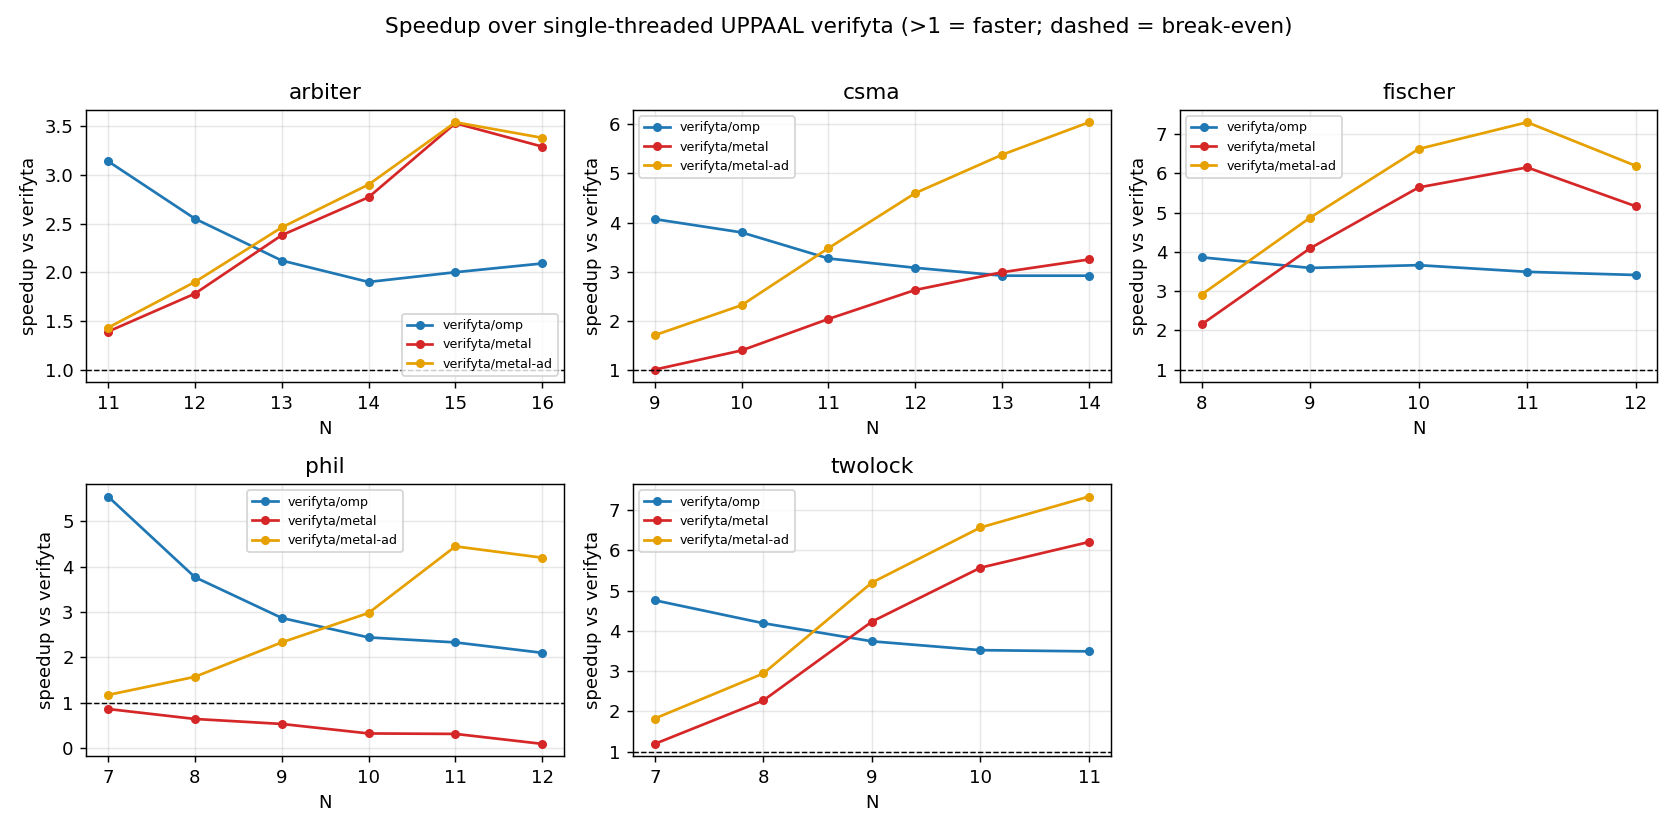
\includegraphics[width=\textwidth]{figs/speedup_vs_verifyta.png}
\caption{Speed-up over single-threaded UPPAAL \code{verifyta} versus model size $N$ (a point above the
dashed line is faster than \code{verifyta}). \code{omp} beats \code{verifyta} on every model;
\code{metal-ad} (adaptive) is above it almost everywhere and is the top line at large $N$, including on
philosophers where the \emph{naive} \code{metal} (not shown here; see \cref{fig:adaptive}) falls below
break-even. (Inflated values at small $N$ are UPPAAL's fixed ${\sim}50$\,ms start-up, negligible at the
sizes that matter---read each curve at its right-hand end.)}
\label{fig:speedup}
\end{figure*}

\paragraph{Naive metal: a win on expansion, a loss on merge.} On Fischer, two-lock and arbiter the
frontier is a large set of mostly-independent zones with small per-key antichains, so runtime is
dominated by the uniform arithmetic of \emph{expansion}---the GPU's strength---and even the naive
\code{metal} beats OpenMP (Fischer/two-lock $N{=}9$--$12$; arbiter $N{=}13$--$16$). But on the
merge-heavy models the naive one-thread-per-bucket merge (\cref{sec:metal}) collapses: on philosophers
the exact convex union fires constantly, and a handful of weak GPU lanes each grind through an
$O(k^2\dim^3)$ per-bucket load while the CPU idles. The effect is dramatic and super-linear---at
philosophers $N{=}12$ the naive Metal merge takes \textbf{122\,s}, an order of magnitude \emph{slower}
than plain \code{seq}. This is the empirical face of the tension in the abstract: expansion is parallel
\emph{across} states, but the merge is sequential \emph{within} a bucket.

\paragraph{Adaptive metal fixes it.} Routing the merge per level (\cref{sec:adaptive})---GPU when
buckets are many and thin, the 12 CPU cores when they are few and fat---turns that loss into the
best result on the board. \Cref{fig:adaptive} plots the ratio: \code{--adaptive} is a
\textbf{$14\times$} speed-up on philosophers $N{=}11$ and a \textbf{$47\times$} speed-up at $N{=}12$
($121.9\!\to\!2.59$\,s), a $1.9\times$ win on CSMA, and---crucially---never a regression on the
already-fast expansion-dominated models (ratio ${\approx}\,1$ on Fischer, two-lock, arbiter, since the
calibration simply leaves the merge on the GPU there). With adaptive on, \code{metal-ad} beats OpenMP
at every large $N$ across \emph{all five} models (\cref{tab:main}).

\begin{figure}[t]
\centering
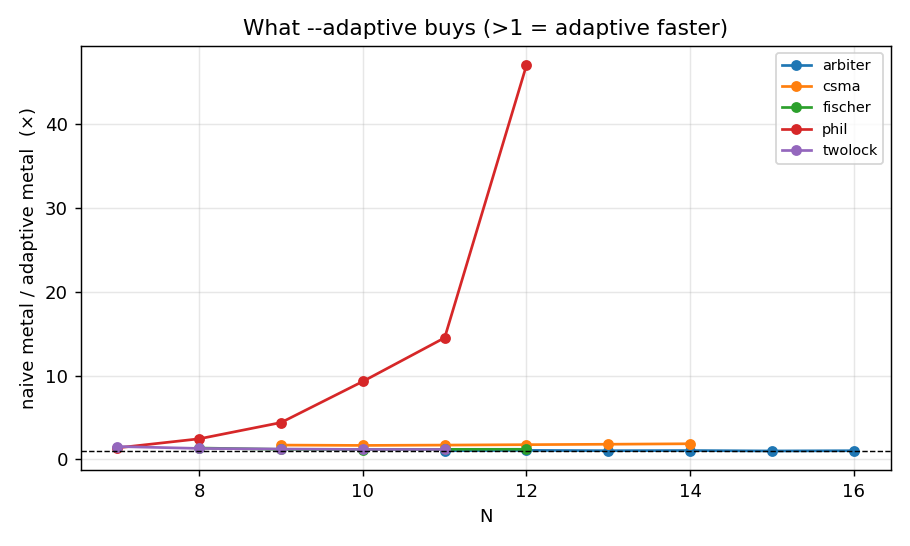
\includegraphics[width=\linewidth]{figs/adaptive_speedup.png}
\caption{What \code{--adaptive} buys: naive-merge time $/$ adaptive-merge time (${>}1$ = adaptive
faster). It is a $47\times$ speed-up on the merge-heavy philosophers at $N{=}12$ and a modest win on
CSMA, while staying ${\approx}1$ (no regression) on the expansion-dominated models---the calibration
routes each level to the faster path.}
\label{fig:adaptive}
\end{figure}

\paragraph{Memory: the honest ceiling.} \Cref{tab:memory,fig:memory} report peak RSS. Ordering is
consistent: \code{seq}\,${\lesssim}$\,\code{omp}\,${<}$\,\code{metal}\,${<}$\,\code{metal-ad}, because
the GPU path double-buffers zones into GPU-facing buffers and the adaptive path adds host merge
buffers on top. UPPAAL is by far the leanest ($0.1$--$0.6$\,GB, an order of magnitude below any
PTCTLMC backend)---its minimal-constraint federations trade time for space, the opposite of our
trade. Memory, not time, is what bounds the largest instances on a $24$\,GB laptop: \code{metal-ad}
reaches ${\sim}13$\,GB at Fischer $N{=}12$, and one step further exhausts RAM for every backend. This
is where a datacentre GPU (\cref{sec:cuda}) with far more memory changes the calculus.

\begin{table}[t]
\centering\small
\caption{Peak resident memory (GB) at the largest timed size. \code{metal-ad} is heaviest (GPU
double-buffering $+$ host merge buffers); \code{verifyta} is an order of magnitude leaner.}
\label{tab:memory}
\begin{tabular}{l r r r r r r}
\toprule
model & $N$ & \code{seq} & \code{omp} & \code{metal} & \code{metal-ad} & \code{vfy} \\
\midrule
Fischer      & 12 & 7.45 & 7.84 & 6.54 & 11.24 & 0.55 \\
two-lock     & 11 & 1.92 & 2.33 & 3.43 & 4.04 & 0.18 \\
arbiter      & 16 & 2.75 & 3.25 & 5.20 & 6.39 & 0.11 \\
CSMA/CD      & 14 & 2.15 & 2.22 & 2.94 & 3.90 & 0.14 \\
philosophers & 12 & 1.35 & 1.82 & 2.31 & 2.72 & 0.19 \\
\bottomrule
\end{tabular}
\end{table}

\begin{figure}[t]
\centering
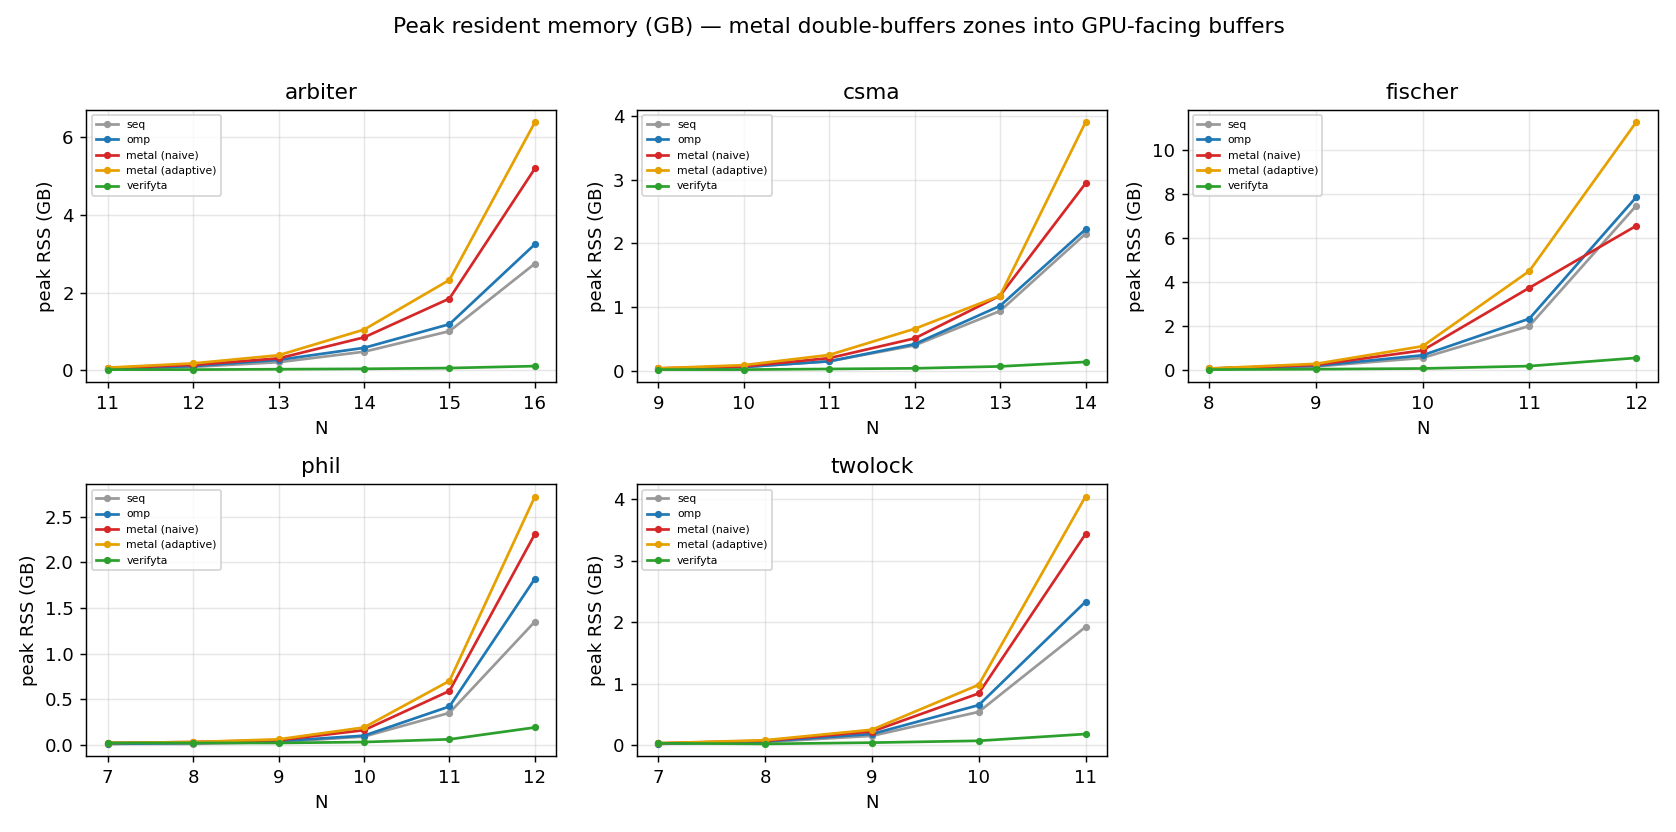
\includegraphics[width=\linewidth]{figs/memory_all.png}
\caption{Peak RSS (GB) vs $N$ per model. The GPU backends carry a memory premium from double-buffering
into unified-memory buffers (adaptive most of all); \code{verifyta} is consistently the leanest. On a
$24$\,GB machine this footprint, not run time, sets the ceiling.}
\label{fig:memory}
\end{figure}

\paragraph{A third negative result: frontier chunking does not buy memory.} Since memory---not
time---is the binding constraint, the obvious lever is to stop materialising a whole BFS level at
once. We added \code{--chunking N}, which expands the frontier in bounded batches so the
unified-memory pools are sized to a \emph{chunk} rather than to the widest level (the frontier is a
worklist, so batching only changes the schedule, never the verdict). It does exactly what it claims at
the level we control: at Fischer $N{=}11$ it cuts the peak expand pool from $1.44$M work items to
$41.6$k, and the summed buffer length from $2.15$\,GB to $0.26$\,GB---an $8\times$ reduction.

\emph{And it does not reduce peak RSS at all} (\cref{tab:chunk}). Worse, small chunks \emph{increase}
it while costing up to $12\times$ in run time. The explanation is the same one that makes the memory
gap hard to close: \code{vmmap} attributes the bulk of the footprint not to our buffers but to
\code{IOAccelerator} regions the Metal driver holds \emph{non-volatile} and reclaims only lazily. A
smaller chunk means \emph{more} levels, hence more per-level transient allocations for the driver to
retain---so the lever we control (pool size) is not the quantity that sets the peak. We keep the flag,
default off, and report it as a negative result: on this runtime, bounding your own allocations is not
sufficient to bound resident memory.

\begin{table}[t]
\centering\small
\caption{Frontier chunking at Fischer $N{=}12$: wall-clock seconds and peak RSS (GB) versus chunk size
(``off'' $=$ \code{metal-ad}). Bounding the GPU pools leaves peak RSS unchanged while run time degrades
sharply, because the resident peak is driver-retained memory, not our buffers.}
\label{tab:chunk}
\begin{tabular}{l r r r r r}
\toprule
chunk (frontier states) & off & $256$k & $64$k & $16$k & $4$k \\
\midrule
wall-clock (s) & \textbf{8.25} & 10.01 & 17.49 & 47.83 & 99.30 \\
peak RSS (GB)  & 11.24 & 11.23 & 11.40 & 11.12 & 11.68 \\
\bottomrule
\end{tabular}
\end{table}

\begin{figure}[t]
\centering
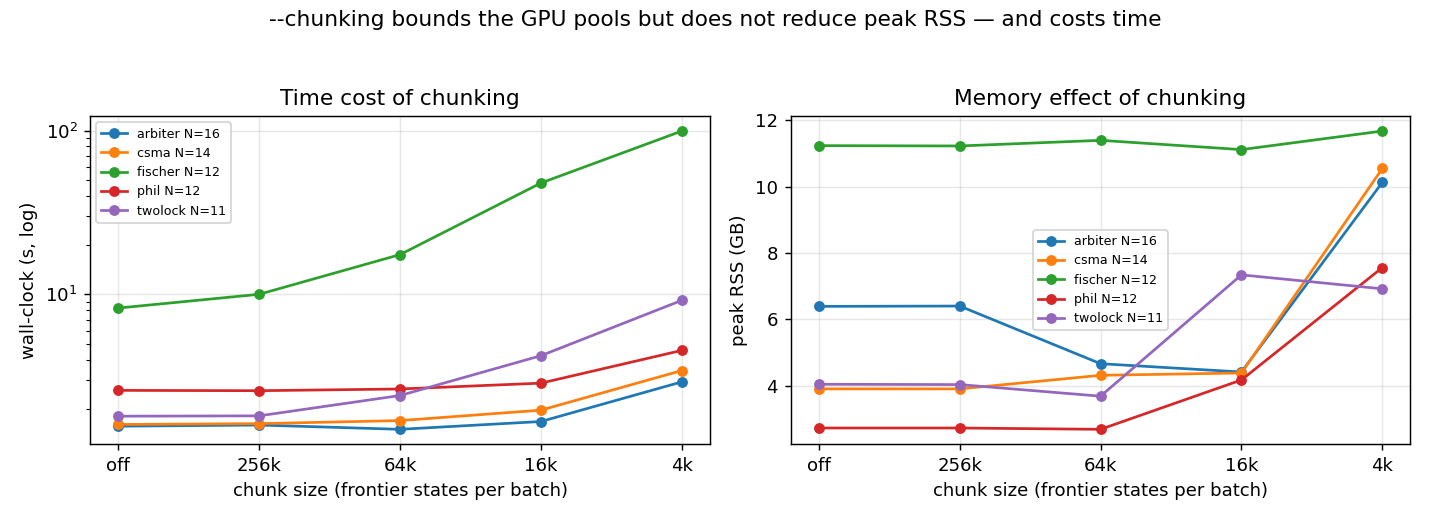
\includegraphics[width=\linewidth]{figs/chunking_tradeoff.png}
\caption{Frontier chunking across all five models (each at its largest $N$). Run time degrades
monotonically as the chunk shrinks (left, log scale) while peak RSS stays flat or gets \emph{worse}
(right). The effect is not model-specific: bounding the pools \emph{we} allocate does not bound what
the GPU driver keeps resident.}
\label{fig:chunk}
\end{figure}

% ===========================================================================
\section{Discussion and conclusion}
% ===========================================================================
Two backends, one control structure, one correctness oracle---and, crucially, one that we hold
honest by matching UPPAAL's explored/stored counts \emph{exactly} (\cref{tab:parity}), so every
speed-up compares like with like. The OpenMP backend earns its speed by \emph{partitioning
ownership} (shard-by-key, lock-free merge) and by \emph{taming the allocator} (per-thread pools).
The Metal backend earns its speed by keeping the GPU busy with the uniform work it likes
(expansion) while a \emph{parallel} host layer feeds it through unified memory with as few copies as
possible---so the whole machine, GPU and all CPU cores, works at once. Every parallel backend beats a
mature single-threaded tool on every model, and the adaptive Metal backend does so by
$3.4$--$7.3\times$ while being the fastest configuration throughout.

The decisive variable is the \emph{ratio of expansion to merge}. Expansion is parallel \emph{across}
symbolic states---the GPU's home turf---but the antichain merge is sequential \emph{within} a
discrete-state bucket, and the GPU merge kernel spends one thread per bucket. When buckets are many
and thin (Fischer, two-lock, arbiter) that is a fine fit and the GPU wins outright; when they are few
and fat (philosophers) a few weak GPU lanes carry the whole load and the naive merge collapses---at
$N{=}12$ it is $47\times$ slower than routing that same merge onto the 12 CPU cores. Rather than guess
which regime a level is in from static bucket statistics (which do not separate the cases), the
\code{--adaptive} driver \emph{measures} both paths' throughput and routes each level to the faster
one; because it lives in the shared driver, the CUDA backend inherits it. That single mechanism turns
the backend's worst case into its best result and leaves the good cases untouched. The remaining
honest limit is \emph{memory}: the GPU backends pay a double-buffering premium (adaptive most of all),
UPPAAL is an order of magnitude leaner, and on a $24$\,GB laptop peak RAM---not run time---is what
caps the largest instances---and \code{--chunking}, which bounds the pools we allocate $8\times$,
does not bound what the driver keeps resident, so it buys no memory and costs time. Two further
attempts to cut the zone traffic (a GPU-resident arena and a direct
frontier buffer) backfired for concrete, measurable reasons. A datacentre GPU
(\cref{sec:cuda})---far more memory and thousands more lanes---is where the same design has the most
room to grow. The broader takeaways transfer well beyond this checker: profile relentlessly, suspect
the memory plumbing before the compute, prefer ownership to locking, \emph{match the parallel
granularity to the data}---and when you cannot predict the right granularity, \emph{measure it at run
time} rather than hard-coding a heuristic.

\end{document}
